\subsection{Experimental Evaluation: UV AMBC}


\begin{frame}[t]{Adaptive Model-Based Control, Overview}%{LS Model Identification}
   \begin{columns}
      \column{.40\textwidth}
    \begin{center}
      \begin{figure}[htbp]
        \begin{center}
          \includegraphics[width=\textwidth]{./pres/images/justJason}
        \end{center}
      \end{figure}
    \end{center}
  \column{.6\textwidth}

   \begin{itemize}
\item<1> 6-DOF UV Model-Based Control (MBC)
\item<1> 6-DOF UV Adaptive Model-Based Control (AMBC)
\item<1-2,4> Experimental Analysis: Thruster Dynamics and AMBC
\item<1,3-4> Experimental Evaluation: UV Two-Step AMBC
   \end{itemize}
\end{columns}

\vskip9pt
\uncover<4>{
  \noindent To simplify and clarify this experimental analysis, we
  will assume the mass and drag matrices are diagonal. This means we
  assume only 16 parameters are required to model UV dynamics: 6
  scalar mass terms (one for each DOF), 6 scalar drag terms (one for
  each DOF), and the previously discussed 3 scalar buoyancy terms and 1
  scalar gravitational term.
}

\end{frame}


% \begin{frame}{Adaptive Model-Based Control Experimental Evaluation}
% %{Parameter Estimate and Trajectory Tracking Evaluation}

% The AMBC experimental evaluation:
% \begin{itemize}
% \item shows how unmodeled thruster dynamics can cause 
%   instability for parameters estimates associated with pitch and roll motion;
% \pause
% \item Discusses a two-step AMBC algorithm which is robust to
%   unmodeled thruster dynamics; and
% \pause
% \item reports a comparative experimental evaluation of PDC and
%   AMBC for simultaneous motion in all DOF.
% \end{itemize}

% \pause
% \vskip9pt
%  To simplify and clarify this experimental analysis, we will
%   assume an uncoupled model of vehicle dynamics. 

%   \pause \vskip9pt JHU ROV control system uses {\it steady-state}
%   assumptions when calculating thruster commands; a common assumption
%   in UV control systems. Unmodeled thruster dynamics is common for UV.
%   The two-step algorithm reported herein could be appropriate for
%   implementing AMBC on vehicles who make these assumptions.


% % {\tiny \setlength\arraycolsep{1pt}

% % \begin{align}
% % M& D_1& D_2& D_3& D_4& D_5& D_6& b& g \nonumber \\
% % \left[\begin{array}{cccccc}
% % \cdot&\cdot&\cdot&\cdot&\cdot&\cdot\\ 
% % \cdot&\cdot&\cdot&\cdot&\cdot&\cdot\\ 
% % \cdot&\cdot&\cdot&\cdot&\cdot&\cdot\\ 
% % \cdot&\cdot&\cdot&\cdot&\cdot&\cdot\\ 
% % \cdot&\cdot&\cdot&\cdot&\cdot&\cdot\\ 
% % \cdot&\cdot&\cdot&\cdot&\cdot&\cdot
% % \end{array}\right] &
% % \left[\begin{array}{cccccc}
% % \cdot&\cdot&\cdot&\cdot&\cdot&\cdot\\ 
% % \cdot&\cdot&\cdot&\cdot&\cdot&\cdot\\ 
% % \cdot&\cdot&\cdot&\cdot&\cdot&\cdot\\ 
% % \cdot&\cdot&\cdot&\cdot&\cdot&\cdot\\ 
% % \cdot&\cdot&\cdot&\cdot&\cdot&\cdot\\ 
% % \cdot&\cdot&\cdot&\cdot&\cdot&\cdot
% % \end{array}\right] &
% % \left[\begin{array}{cccccc}
% % \cdot&\cdot&\cdot&\cdot&\cdot&\cdot\\ 
% % \cdot&\cdot&\cdot&\cdot&\cdot&\cdot\\ 
% % \cdot&\cdot&\cdot&\cdot&\cdot&\cdot\\ 
% % \cdot&\cdot&\cdot&\cdot&\cdot&\cdot\\ 
% % \cdot&\cdot&\cdot&\cdot&\cdot&\cdot\\ 
% % \cdot&\cdot&\cdot&\cdot&\cdot&\cdot
% % \end{array}\right] &
% % \left[\begin{array}{cccccc}
% % \cdot&\cdot&\cdot&\cdot&\cdot&\cdot\\ 
% % \cdot&\cdot&\cdot&\cdot&\cdot&\cdot\\ 
% % \cdot&\cdot&\cdot&\cdot&\cdot&\cdot\\ 
% % \cdot&\cdot&\cdot&\cdot&\cdot&\cdot\\ 
% % \cdot&\cdot&\cdot&\cdot&\cdot&\cdot\\ 
% % \cdot&\cdot&\cdot&\cdot&\cdot&\cdot
% % \end{array}\right] &
% % \left[\begin{array}{cccccc}
% % \cdot&\cdot&\cdot&\cdot&\cdot&\cdot\\ 
% % \cdot&\cdot&\cdot&\cdot&\cdot&\cdot\\ 
% % \cdot&\cdot&\cdot&\cdot&\cdot&\cdot\\ 
% % \cdot&\cdot&\cdot&\cdot&\cdot&\cdot\\ 
% % \cdot&\cdot&\cdot&\cdot&\cdot&\cdot\\ 
% % \cdot&\cdot&\cdot&\cdot&\cdot&\cdot
% % \end{array}\right] &
% % \left[\begin{array}{cccccc}
% % \cdot&\cdot&\cdot&\cdot&\cdot&\cdot\\ 
% % \cdot&\cdot&\cdot&\cdot&\cdot&\cdot\\ 
% % \cdot&\cdot&\cdot&\cdot&\cdot&\cdot\\ 
% % \cdot&\cdot&\cdot&\cdot&\cdot&\cdot\\ 
% % \cdot&\cdot&\cdot&\cdot&\cdot&\cdot\\ 
% % \cdot&\cdot&\cdot&\cdot&\cdot&\cdot
% % \end{array}\right] &
% % \left[\begin{array}{cccccc}
% % \cdot&\cdot&\cdot&\cdot&\cdot&\cdot\\ 
% % \cdot&\cdot&\cdot&\cdot&\cdot&\cdot\\ 
% % \cdot&\cdot&\cdot&\cdot&\cdot&\cdot\\ 
% % \cdot&\cdot&\cdot&\cdot&\cdot&\cdot\\ 
% % \cdot&\cdot&\cdot&\cdot&\cdot&\cdot\\ 
% % \cdot&\cdot&\cdot&\cdot&\cdot&\cdot
% % \end{array}\right] &
% % \left[\begin{array}{cccccc}
% % \cdot&\cdot&\cdot&\cdot&\cdot&\cdot\\ 
% % \cdot&\cdot&\cdot&\cdot&\cdot&\cdot\\ 
% % \cdot&\cdot&\cdot&\cdot&\cdot&\cdot\\ 
% % \cdot&\cdot&\cdot&\cdot&\cdot&\cdot\\ 
% % \cdot&\cdot&\cdot&\cdot&\cdot&\cdot\\ 
% % \cdot&\cdot&\cdot&\cdot&\cdot&\cdot
% % \end{array}\right]
% % \left[\begin{array}{c}
% % \cdot\\
% % \cdot\\
% % \cdot
% % \end{array}\right] &
% % \left[\begin{array}{c}
% % \cdot
% % \end{array}\right] 
% % \nonumber
% % \end{align}
% % }


% % \begin{columns}
% %   \column{.57\textwidth} \alert<1-2>{Our Goal}: Evaluate if the
% %   parameter estimation process is stable, if UV AMBC is better than UV
% %   proportional derivative control (PDC), and 
  
% %       adaptive identification and least squares identification
% %       \alert<2>{provide similar capacity to model vehicle dynamics}.

% %       \vskip10pt

% %       \begin{itemize}
% %       \item<3-> Run eight experiments 
% %        \begin{itemize}
% %        \item<3-> Using simplified model 
% %        \item<3->
% %        \end{itemize}
% %      %\item<4-> Evaluation process used for \alert<6->{both Least
% %      %    Squares and Adaptive Identification}
% %      \item<4-> Compare state measurements from second experiment 
% %                to state estimates from UV forward simulation
% %       \item<5-> Mean Absolute Error (MAE) between measured and
% %         simulated vehicle states used to judge modeling accuracy

% %       \end{itemize} 
    
% %     \column{.43\textwidth}
% %      \only<4->{
% %       \begin{center}
% %         \begin{figure}[htbp]  
% %           \begin{center}
% % %            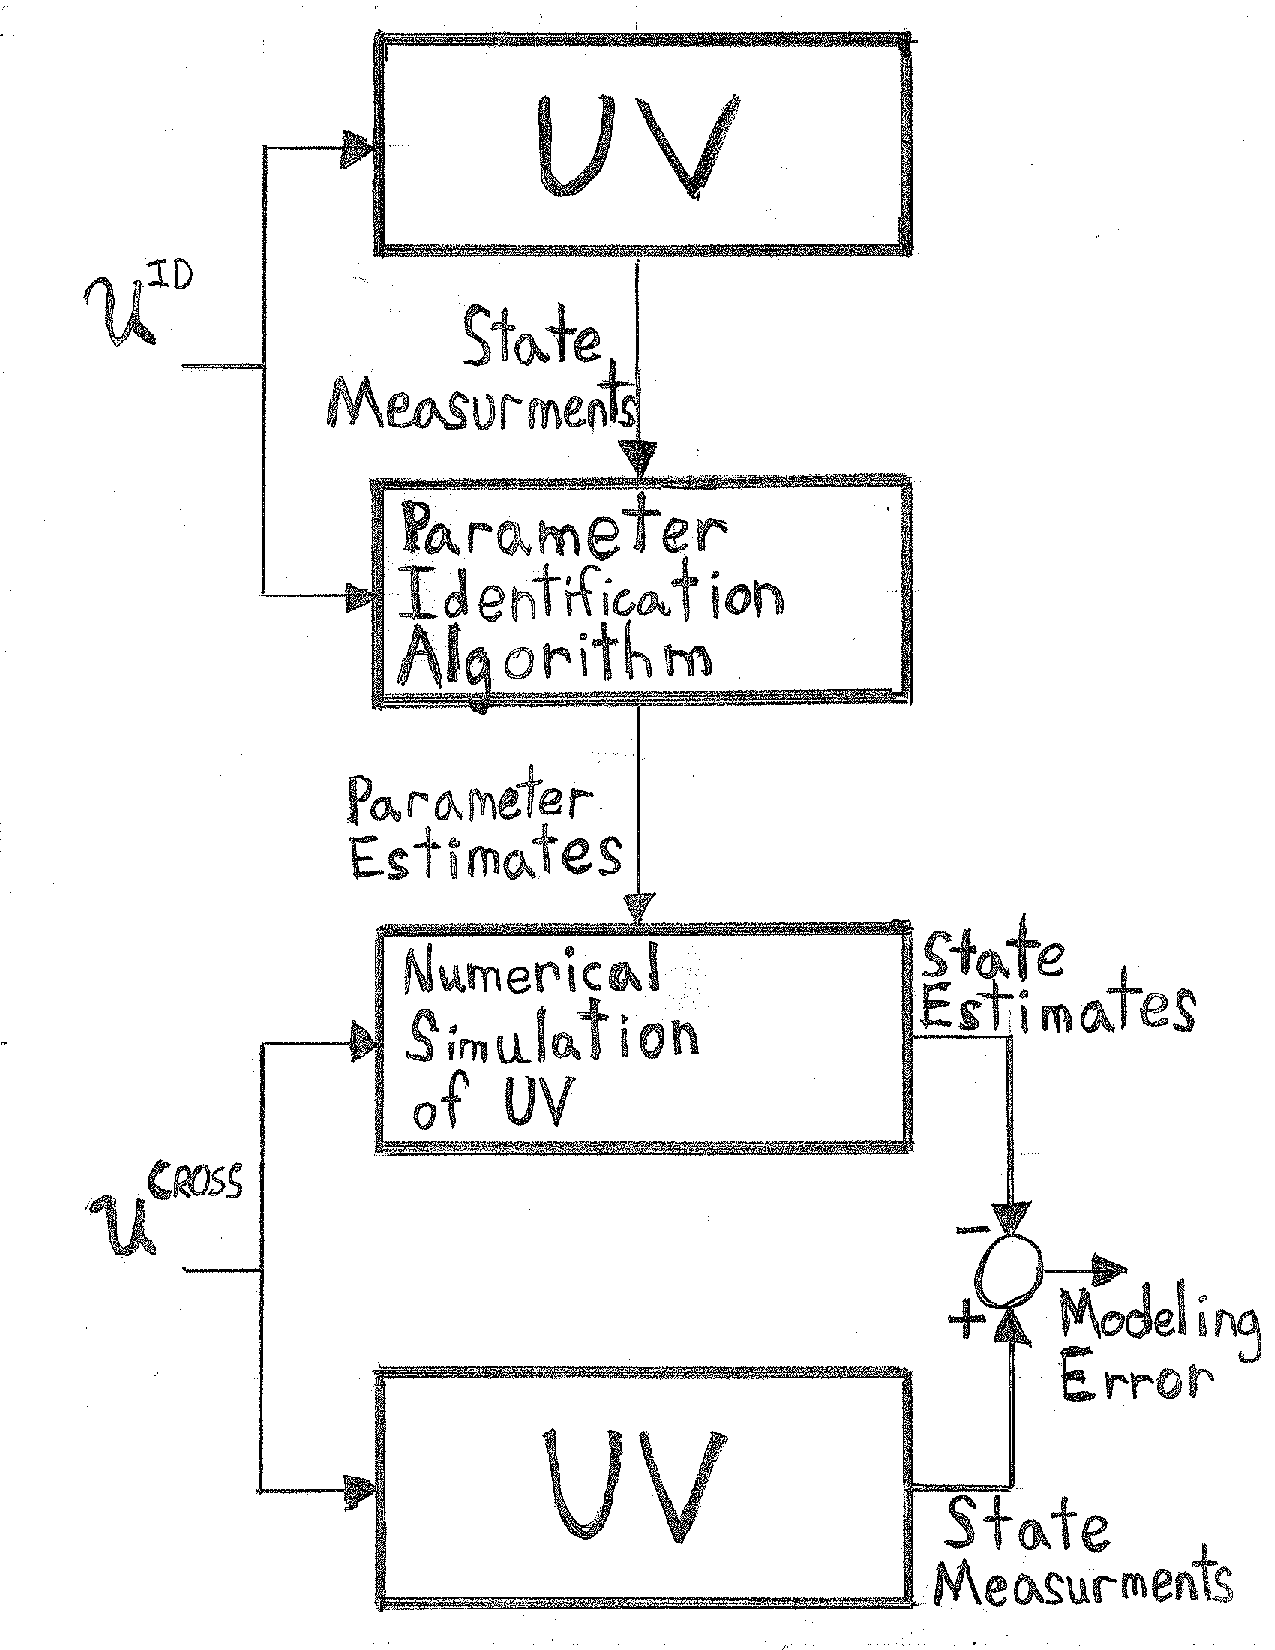
\includegraphics[width=50mm]{./pres/images/blockDiaSketch}
% %           \end{center}
% %         \end{figure}
% %       \end{center}    
% %       }
% %   \end{columns} 

% \end{frame}




%\begin{frame}{Instability Indicators: What Does Parameter Estimate Instability Look Like?}
\begin{frame}{Expt A: AMBC {\it failure }Experimental Evaluation}

\begin{itemize}
\item<1->\alert<1-4>{Problem 1:} %{Indicator 1:}  
 When initialized to
  physically realistic values, parameters adapt to physically
  unrealistic values.
\item<2-4>Consider the initial and final parameter estimates from an
  experiment where AMBC tracks a 6 DOF reference trajectory:
\begin{itemize}
\item<3-4> Most parameter estimates oscillate around initial values. (That's good)
\item<4>$\hat{m}_4(t)$ and $\hat{m}_5(t)$ adapted towards negative values.  (That's bad)
\end{itemize}
\item<5->\alert<5->{Problem 2:} %{Indicator 2:} 
Parameter estimates do
  not display asymptotic behavior.
\begin{itemize}
\item<6->$\hat{m}_4(t)$ and $\hat{m}_5(t)$ show no signs of asymptotic
  behavior.
\end{itemize}
\end{itemize}


\alt<1>{\vspace*{45mm}}{
\alt<1-5>{%\small

\begin{table}[htbp]
%\ssp
%\caption{Mass and Drag Parameters Identified During Unstable Parameter Adaptation}
\begin{center}
\begin{tabular}{c|cccc}
 & $m_i(t_o)$ & $m_i(t_f)$ & $d_i(t_o)$ & $d_i(t_f)$ \\ \hline
Trans X DOF & 583 {\it kg} & 583 {\it kg}& -1245 {\it $\frac{\text{N}~\text{s}^2}{\text{m}^2}$}& -1005 {\it $\frac{\text{N}~\text{s}^2}{\text{m}^2}$}\\
Trans Y DOF & 873 {\it kg} & 769 {\it kg}& -1426 {\it $\frac{\text{N}~\text{s}^2}{\text{m}^2}$}& -1400 {\it $\frac{\text{N}~\text{s}^2}{\text{m}^2}$}\\
Trans Z DOF & 1021 {\it kg} & 1031 {\it kg}& -3060 {\it $\frac{\text{N}~\text{s}^2}{\text{m}^2}$}& -3039 {\it $\frac{\text{N}~\text{s}^2}{\text{m}^2}$}\\
Angular X DOF & \alert<4>{103.5 {\it kg $\text{m}^2$}} & \alert<4>{-1.348 {\it kg $\text{m}^2$}} & -728.4 {\it N $\text{s}^2$}& -761.5  {\it N $\text{s}^2$}\\
Angular Y DOF & \alert<4>{137.1 {\it kg $\text{m}^2$}} & \alert<4>{42.5 {\it kg $\text{m}^2$}} & -769.1  {\it N $\text{s}^2$}& -681.4  {\it N $\text{s}^2$}\\
Angular Z DOF & 106.4 {\it kg $\text{m}^2$} & 41 {\it kg $\text{m}^2$} & -376.2  {\it N $\text{s}^2$}& -393.3  {\it N $\text{s}^2$}\\
\end{tabular}
\end{center}
\vskip9pt
\vskip9pt
%\label{chUV_AMBC.tb.startCloseDyn}
%\vspace*{-5mm}
\end{table}
}{
\begin{center}
\begin{figure}[htbp]
  \begin{center}
    \includegraphics[width=.9\textwidth]{./chUV_AMBC/images/m4_m5_Full_Param_EstSm}
  \end{center}
%  \caption{ The time evolution of Angular X DOF and Angular Y
%    DOF mass estimates from \ac{AMBC} during 6-DOF dynamic
%    maneuvers. These mass estimates adapt to physically unrealistic
%    negative values and show no signs of asymptotic behavior.}
%  \label{chUV_AMBC.fig.m4_m5_Full_Param_Est}
%\vspace*{-5mm}
\end{figure}
\end{center}
}}

\end{frame}




%\begin{frame}{Thrust Reversals Lead to Unstable Parameter Adaptation?}
\begin{frame}{Expt B: Thrust Reversals Lead to Unstable Parameter Adaptation}

  A pitch-only AMBC experiment shows how \alert<2-3>{commanded thrust
    reversals} lead to \alt<3>{\color{blue}unmodeled thruster
    dynamics}{unmodeled thruster dynamics} which
  \alt<5>{\color{green}destabilizes}{destabilizes} parameter adaptation.

\begin{columns}
  \column{.5\textwidth} 


      \begin{center}
\alt<1>{\vspace*{30mm}}{ 
        \begin{figure}[htbp]  
          \begin{center}
            \includegraphics[width=\textwidth]{./chUV_AMBC/images/stictionErrorWithThrustReversals}
          \end{center}
        \end{figure}}
      \end{center}   

    
    \column{.5\textwidth}
      \begin{itemize}
 %     \item<1-> Commanded and Estimated Thrust shown for thrusters controlling vehicle pitch 
      \item<2-> After \alert<2-3>{thrust reversal}: \alt<3>{\color{blue}commanded thrust
        $0\text{ N}\leq u_i\leq 5$ N, estimated thrust $0$ N}{commanded thrust
        $0\text{ N}\leq u_i\leq 5$ N, estimated thrust $0$ N}
    \item<4-> AMBC interprets position and velocity deviations as the
      pitch mass estimate is too large
    \item<5->Pitch mass estimate update law has \alt<5>{\color{green}negative
        spike}{negative spike}
       \item<6->Pitch mass estimate adapts to physically unrealistic value
      \end{itemize} 
    
      \begin{center}
\alt<1-5>{\vspace*{15mm}}{\begin{figure}[htbp]  
          \begin{center}
            \includegraphics[width=\textwidth]{./pres/images/m5_Thrust_Rev_Param_EstSm}
          \end{center}
        \end{figure}}
      \end{center}    
      
  \end{columns} 


\end{frame}

\begin{frame}{Expt C: Stable Parameter Adaptation Without Thrust Reversals}
  For pitch-only AMBC experiment \alert<2-3>{without commanded thrust
    reversals} \alt<3>{\color{green}parameter adaptation is
    stable}{parameter adaptation is stable}.

\begin{columns}
  \column{.5\textwidth} 
 
      \begin{center}
\alt<1>{\vspace*{50mm}}{ 
        \begin{figure}[htbp]  
          \begin{center}
            \includegraphics[width=\textwidth]{./chUV_AMBC/images/stictionErrorWoThrustReversals}
          \end{center}
        \end{figure}}
      \end{center}    

    
    \column{.5\textwidth}
      \begin{itemize}
 %     \item<1-> Commanded and Estimated Thrust shown for thrusters controlling vehicle pitch 
      \item<2->\alert<2>{No thrust reversals}
      \item<3->Without thrust reversals, velocity and position
        deviations and negative spike in the pitch mass estimate
        update law \alt<3>{\color{green}do not occur}{do not occur}
       \item<4->Pitch mass adaptation stable
      \end{itemize} 
    
      \begin{center}
\alt<1-3>{\vspace*{15mm}}{\begin{figure}[htbp]  
          \begin{center}
            \includegraphics[width=\textwidth]{./pres/images/m5_Thrust_No_Rev_Param_EstSm}
          \end{center}
        \end{figure}}
      \end{center}    
      
  \end{columns} 


\end{frame}


\begin{frame}{Unmodeled Thruster Dynamics and Two-Step AMBC}

\begin{itemize}
%\item<1-> JHU ROV control system uses {\it steady-state} assumptions when
%  calculating thruster commands; a common assumption in UV control
%  systems.
%\item<2-> The data suggests thruster dynamics unmodeled by {\it
%    steady-state} models cause unstable parameter adaptation
%  exclusively in the pitch and roll DOF.
\item<1-> The data suggests unmodeled thruster dynamics during thrust
  reversals cause unstable parameter adaptation for parameters
  associated in the pitch and roll DOF.
\item<2-> The effects of unmodeled thruster dynamics are the same on
  buoyancy and mass estimate adaptation; this allows simultaneous
  unstable adaptation in both parameters.
\item<3-> Separately identifying mass and buoyancy parameters
  \alert<4>{COULD} prevent unstable pitch and roll parameter
  adaptation.
\item<5-> Based on UV dynamic equations it is possible to divide the
  parameter estimation process into two successive experimental trials.
\item<6->\alert<6->{Two-Step AMBC}: 
\begin{itemize}
\item<6-> First step estimates buoyancy and gravitational parameters using
  quasi-static roll and pitch reference-trajectory. 
\item<6-> Second step estimates mass and drag parameters \alert<7->{for
    any reference-trajectory}.
\end{itemize}
\end{itemize}



\end{frame}



\begin{frame}{Expt C: Two-Step AMBC Parameter Adaptation is Stable}


\begin{itemize}
\item<1->Consider the initial and final parameter estimates from the second step AMBC
  algorithm tracking a 6 DOF reference trajectory:
\begin{itemize}
\item<2->All parameter estimates were initialized zero.
\item<3->All parameter estimates converge to physically realistic values (that's good!)
\item<4->In cross-validation experiment, AMBC identified models get better at
  modeling vehicle performance through the adaptation process
\end{itemize}
\end{itemize}

\alt<2->{
\alt<1-3>{
%\vskip15pt
\begin{table}[htbp]
\caption{Parameters Identified with 
     two-step AMBC during Dynamic Motion Trajectory-Tracking}
\begin{center}
\begin{tabular}{c|cccc}
 & $m_i(t_o)$ & $m_i(t_f)$ & $d_i(t_o)$ & $d_i(t_f)$ \\ \hline
Trans X DOF & \alert<2>{0.0} {\it kg}& 628 {\it kg}& \alert<2>{0.0} {\it $\frac{\text{N}~\text{s}^2}{\text{m}^2}$}& -1259 {\it $\frac{\text{N}~\text{s}^2}{\text{m}^2}$}\\
Trans Y DOF & \alert<2>{0.0} {\it kg}& 791 {\it kg}& \alert<2>{0.0} {\it $\frac{\text{N}~\text{s}^2}{\text{m}^2}$}& -1429 {\it $\frac{\text{N}~\text{s}^2}{\text{m}^2}$}\\
Trans Z DOF & \alert<2>{0.0} {\it kg}&1043 {\it kg}& \alert<2>{0.0} {\it $\frac{\text{N}~\text{s}^2}{\text{m}^2}$}& -3083 {\it $\frac{\text{N}~\text{s}^2}{\text{m}^2}$}\\
Angular X DOF & \alert<2>{0.0} {\it kg $\text{m}^2$}& \alert<3>{95.7} {\it kg $\text{m}^2$}& \alert<2>{0.0} {\it N $\text{s}^2$}& -727.1 {\it N $\text{s}^2$}\\
Angular Y DOF & \alert<2>{0.0} {\it kg $\text{m}^2$}& \alert<3>{145.3} {\it kg $\text{m}^2$}& \alert<2>{0.0} {\it N $\text{s}^2$}& -783.4 {\it N $\text{s}^2$}\\
Angular Z DOF & \alert<2>{0.0} {\it kg $\text{m}^2$}& 110.2 {\it kg $\text{m}^2$}& \alert<2>{0.0} {\it N $\text{s}^2$}& -465.6 {\it N $\text{s}^2$}\\
\end{tabular}
\end{center}
\end{table}
}{
\vspace*{3mm}
\vskip9pt
{\scriptsize
\begin{table}[htbp]
\caption{Mean Absolute Error Values Comparing Simulated and Measured Vehicle Performance for Cross-Validation Experiment}
\begin{center}
\begin{tabular}{p{1.5cm}|cccccccc}
Time of AMBC & \multicolumn{2}{c}{Angular Pose ($^\circ$)} & \multicolumn{3}{c}{Translational Velocity (m/s) }& \multicolumn{3}{c}{Angular Velocity ($^\circ$/s)} \\ 
Parameter Set & Roll & Pitch & x DOF & y DOF & z DOF & x DOF & y DOF & z DOF \\ \hline
250 sec      &  2.6 & 2.2 & 0.102  & 0.107  & 0.35  & 2.3 & 2.4 & 4.3 \\
1000 sec     &  2.2 & 1.81 & 0.048  & 0.042 & 0.138  & 1.77 & 1.48 & 3.6 \\
5000 sec     & 1.06 & 1.1 & 0.039  & 0.042  & 0.035 & 1.34 & 0.89 & 2.8 \\
\end{tabular}
\end{center}
\end{table}}
\vskip9pt
\vskip9pt
\vskip9pt
\vskip9pt
}}{\vspace*{47mm}}

\end{frame}


% \begin{frame}{Forward simulation of two-step AMBC identified models}

% \begin{columns}
%     \column{.5\textwidth}

%      \begin{center}
%         \begin{figure}[htbp]  
%           \begin{center}
%             \includegraphics[width=.8\textwidth]{./chUV_AMBC/images/OLO_All}
%           \end{center}
%         \end{figure}
%       \end{center}    

%     \column{.5\textwidth}

% \begin{itemize}
% \item Experimentally measured states verses the states from numerical
%   simulations; each numerical simulation uses a model identified by
%   the two-step AMBC after a set amount of time.
% \item parameter estimates are progressively improving at modeling JHU ROV performance
% \item The states shown from simulating the ``5000
% sec'' parameter set indicate that AMBC can produce parameter estimates
% which result in accurate plant models.
% \end{itemize}

% \vskip9pt
% \vskip9pt
% \vskip9pt
% \vskip9pt
% \vskip9pt
% \vskip9pt

% \end{columns}


% \end{frame}



%\begin{frame}{Two-Step AMBC}
%
%\end{frame}





\begin{frame}{Expt C: Two-Step AMBC vs PDC Comparative Experimental Analysis}

\begin{itemize}
%\item<1->PDC tracking performance compared to second-step AMBC
%  tracking performance with the same PD gains and reference trajectory
\item<2->Mean normalized of errors vectors (MNE) for
  position and velocity
\begin{itemize}
\item<3->PDC MNE values calculated using 10 minutes of data%,  plotted in green 
\item<4->AMBC MNE values calculated for consecutive 15 minute windows%, plotted in blue
\end{itemize}
\item<5->After parameter convergence the two-step AMBC provides
$30\%$ better position tracking and $8\%$ worse velocity tracking.
\end{itemize}

\begin{center}
\begin{figure}[htbp]
  \begin{center}
    \includegraphics[width=.8\textwidth]{./chUV_AMBC/images/MNE_All}
  \end{center}
\end{figure}
\end{center}

\end{frame}


